\chapter{Exercise 2}

\section{Question 1}
We compute the optimal portfolio for an investor using Markowitz' formula. We assume that the investor seeks to maximize the following expected utility function:
\begin{equation*}
\max_\omega E\left[-e^{-\lambda X}\right]
\end{equation*}
where $X$ represents the expected returns and it is a random variable following the normal distribution with $N(\mu, \Sigma)$, where $\Sigma$ is the covariance matrix. Using the Laplace transform, we can rewrite it as

\begin{equation*}
\max_\omega E\left[-e^{{-\lambda \omega^T+}\frac{1}{2}\lambda^2\omega^T\Sigma\omega}\right]
\end{equation*}
From the first order conditions we get that the optimal weight allocation on the different investment possibilities is given by the vector
\begin{equation*}
\omega = \frac{1}{\lambda}\Sigma^{-1}\mu
\end{equation*}

\section{Question 2}

We have calculated the performance of the portfolio as $\mu^T\omega$ with variance $\omega^T\Sigma\omega$, which for our data is: \bigskip

Expected return on the portfolio: 0.0536

Variance of the portfolio: 0.01788 \bigskip

Figure \ref{fig4} shows the distribution of the performance. Compound and average returns can produce very different results over time, as we can see in our graph there are ups and downs, that means that our investment in the portfolio don’t always give us the average rate of return every period but rather an average desired rate of return on a given period. The weights on the portfolio will also depend on the risk-aversion factor that the investor “has”.

\begin{figure}[ht]
\centering
\includegraphics[width=10cm, angle=270]{Q2_2plot.eps}
\caption{Expected performance of the optimal portfolio}
\label{fig4}
\end{figure}
